\documentclass[conference,10pt,letterpaper,twoside]{ieeeconf}

\IEEEoverridecommandlockouts

% to use ieeeconf with natbib
\makeatletter
\let\NAT@parse\undefined
\makeatother

\usepackage[numbers,sort,compress]{natbib}

\usepackage{graphicx}
\usepackage{color}
\usepackage{multirow}
\usepackage{balance}

\usepackage{amsmath,amssymb} % define this before the line numbering.
\usepackage{mathtools}
\usepackage{algorithmic}
\usepackage{algorithm}

\usepackage{caption}
%\usepackage[skip=0pt]{subcaption}
\usepackage{subcaption}
\captionsetup{
   labelfont = small,%footnotesize,
   textfont = small,%footnotesize,
   %skip = 1ex,  % skip the space between float and caption
   %belowskip=-10pt,
}

% perls packages
\usepackage{perl_acronyms}
\usepackage{perl_math}
\usepackage{perl_SIunits}
\usepackage{perl_misc}


\definecolor{jgreen}{RGB}{0,155,0}
\definecolor{ared}{RGB}{155,0,0}
\newcommand{\jmw}[1]{{\color{jgreen}[}jmw:\ {\color{jgreen}#1]}}
\newcommand{\aku}[1]{{\color{ared}[}aku:\ {\color{ared}#1]}}


\title{Object Detection using a Probabilistic Ray-Based Observation Model}

\author{Arash~K.~Ushani}

\begin{document}

\maketitle

\section{Detection Likelihood Map}\label{sec:dlm}

Our goal is to compute a detection map that captures how likely it is for an
object to exist at a particular location in the world. As our work is targeted
for applications with autonomous vehicles, for runtime performance, we make the
assumption that the world is 2.5D. Namely, we assume that all objects exist on a
horizontal plane and their pose can be fully described by their 2D location and
rotation. However, we fully model the 3D nature of the sensor observations.

We receive a set of \ac{LIDAR} observations, $\mathbf{Z} = \{z_{1:n_z}\}$. Given
these, we evaluate:
%
\begin{align}
  p(\mathrm{obj_{c, x}}| \mathbf{Z}) \text{,} \label{eq:detection_map}
\end{align}
%
where $\mathrm{obj_{c, x}}$ denotes the presence of an object of class $c$ with
pose $x$. As we focus on KITTI, the classes we are concerned with are Car,
Pedestrian, and Cyclist. Additionally, we model a Background class as well. We
refer to \eqref{eq:detection_map} as a probabilistic detection map. Our goal is
to evaluate and generate this map.

Applying Bayes' rule, we have:
%
\begin{align}
  p(\mathrm{obj_{c, x}} | \mathbf{v}) &=
    \frac
      {p(\mathrm{obj_{c, x}}) p(\mathbf{Z} | \mathrm{obj_{c, x}})}
      {p(\mathbf{Z})}
  \text{,}
  \label{eq:bayes}
\end{align}
%
where $p(\mathrm{obj_{c, x}})$ is an object prior,
$p(\mathbf{Z} | \mathrm{obj_{c, x}})$ is the observation model, and
$p(\mathbf{Z})$ is a normalization factor.

The key part of \eqref{eq:bayes} is the observation model. We require an
observation model that is expressive enough to detect objects and differentiate
between different classes. At the same time, we must be able to evaluate this
model quickly for different classes and poses so that it is tractable to
evaluate \eqref{eq:bayes} for a large number of object poses and classes to
fully build the detection map.

\section{Observation Model}

Consider $p( z_i | obj)$. We will assume that $\theta_i$ is known, and thus we
just need to model $p( r_i | obj, \theta_i)$. We will do this by building a
lookup table of histograms from simulated data.

We generate a number of simulated environments with objects placed in random
positions and orientations. We then generate simulated LIDAR data from this
environment.

We take each $z_i$ generated. We project each ray into the object's frame. We
compute the relative angle between the ray and the object, $\phi = \theta_i -
\theta_{object}$. We also compute the closest distance between the ray and the
center of the object location, $d_{\text{ray}}$. Finally, we compute
$d_{\text{obs}}$, the position of the range $r_i$ along the ray, relative to the
closest point along the ray to the object center. This is depicted in
\figref{fig:obs_model}.
%
\begin{figure}
  \centering
  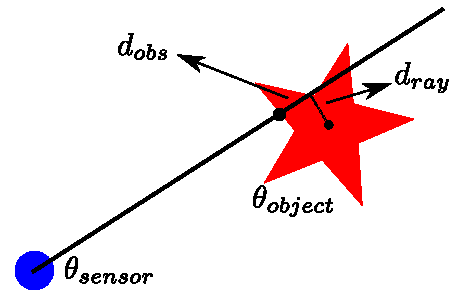
\includegraphics[width=2in]{figures/ray_model.pdf}
  \caption{Ray-based observation model for a given object. The sensor is
    depicted by the blue circle. The red star depicts the object we are
    interested in.}
  \label{fig:obs_model}
\end{figure}
%
Thus, $(\phi, d_{\text{ray}})$ parameterizes the ray for the $z_i$ that we are
considering, and $d_{\text{obs}}$ represents the observation, relative to the
object's location. (Note that these can be positive or negative). So, we have
%
\begin{align}
  p( r_i | obj, \theta_i) &=
    p_{obj}( d_{\text{obs}} | \phi, d_{\text{ray}} )
  \text{.}
\end{align}

We maintain a two-dimensional array of histograms, parameterized by $(\phi,
d_{\text{ray}})$. We discretize $\phi$ at \unit{0.05}{\rad} and
$d_{\text{ray}}$ at \unit{0.05}{\m}. For each $z_i$, we find the appropriate
histogram and update it with $d_{\text{obs}}$.

Additionally, we use negative mining in a similar fashion to estimate
$p( r_i | \lnot obj, \theta_i) = p_{\lnot obj} ( d_{\text{obs}} | \phi, d_{\text{ray}}) $.

Thus, \eqnref{eq:obj_model} becomes:
%
\begin{align}
  \log p( obj | \mathbf{Z} ) &=
   \log{\eta} + \sum_{i=1}^{n} { \log p_{obj}( d_{\text{obs}} | \phi, d_{\text{ray}}) }
   \text{,}
   \label{eq:obj_model_pos}
\end{align}
%
and we also have:
%
\begin{align}
  \log p( \lnot obj | \mathbf{Z} ) &=
   \log{\eta} + \sum_{i=1}^{n} { \log p_{\lnot obj} ( d_{\text{obs}} | \phi, d_{\text{ray}}) }
   \text{.}
   \label{eq:obj_model_neg}
\end{align}

So, by leveraging these observation models, we can compute:
%
\begin{align}
  s_{ \text{obj} }     &=
    \sum_{i=1}^{n} { \log p_{obj}( d_{\text{obs}} | \phi, d_{\text{ray}}) } \\
  s_{\lnot \text{obj}} &=
    \sum_{i=1}^{n} { \log p_{\lnot obj} ( d_{\text{obs}} | \phi, d_{\text{ray}}) } \\
  p ( obj | \mathbf{Z} ) &=
    \frac{1}{1 + \exp{(s_{\lnot \text{obj}} - s_{\text{obj}})}}
  \text{.}
  \label{eq:detection_prob}
\end{align}

To visualize our observation model and verify that it is capturing the right
thing, we can use it to generated a synthetic LIDAR scan of a object. We place
an object at $(0.0, 5.0)$ with $\theta = \unit{18}{\degree}$. For a range of
sensor angles $\theta_i$, we can evaluate $p( r_i | obj, \theta_i ) $ and thus
generate a synthetic scan that represents what we might expect to see. We depict
this in \figref{fig:synthetic_scan} evaluated at different percentiles (e.g., at
50\% we have the median observation we would expect).
%
\begin{figure}
  \centering
  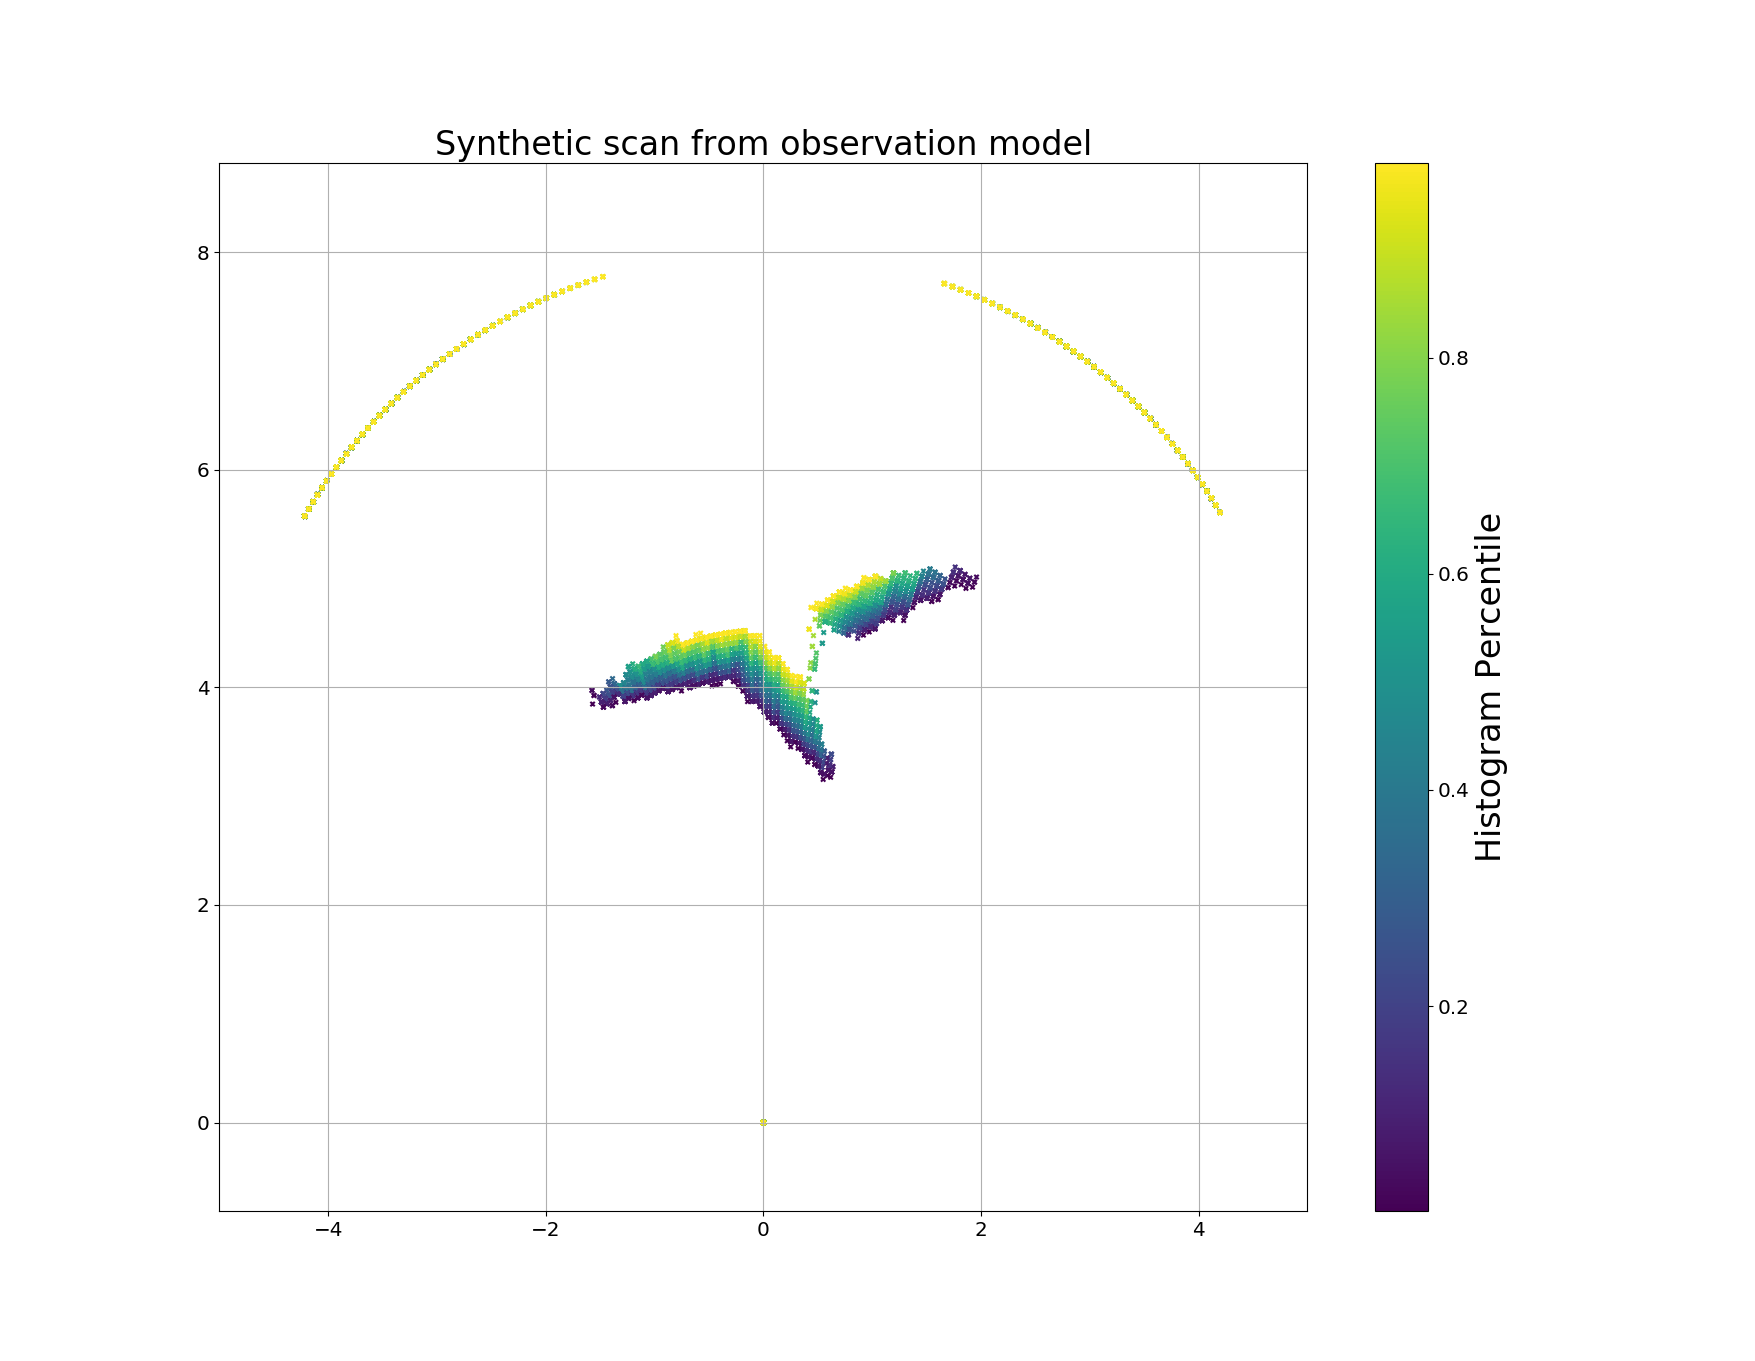
\includegraphics[width=\columnwidth]{figures/synthetic_scan.png}
  \caption{Synthetic scan created for an object at $(0.0, 5.0)$ with $\theta =
    \unit{18}{\degree}$.}
  \label{fig:synthetic_scan}
\end{figure}

\section{Dependence}

Recall that in \eqref{eq:cond_ind} we assumed conditionally independent observations
given the object (namely, its position and class):
%
\begin{align}
  p( \mathbf{Z} | obj_c ) &= \prod_{i=1}^{n} { p( z_i | obj_c) }
  \text{.}
\end{align}
%
However, this is not the case. Consider intraclass variation of objects. A star
object might not always have the same size. In this case, one observation might
capture some of this variation, and thus be informative for the next
observation. For example, if a LIDAR observation is closer to use, that might
indicate that the object is on the large size, and thus the next observation is
likely to be close as well.

Ideally, we would capture the full distribution $p ( \mathbf{Z} | obj_c )$. However,
this is not tractable. We find that making the conditionally independent
assumption hinders the quality of multiclass detection, as it is easy to confuse
different classes. We compromise by creating a "2-gram" model:
%
\begin{align}
  p( \mathbf{Z} | obj_c ) &= \left( \prod_{i=2}^{n} { p( z_i | obj_c, z_{i-1}) }
  \right) p( z_1 | obj_c)
  \text{,}
\end{align}
%
where each observation depends only on the one directly preceding it (note that
with this terminology, we refer to the previous model as the "1-gram" model).
Generally speaking, we can construct this sort of $n$-gram model for any $n$,
but as $n$ grows the distribution quickly becomes more challenging to capture
with simulated training data.

\begin{figure*}
  \centering
  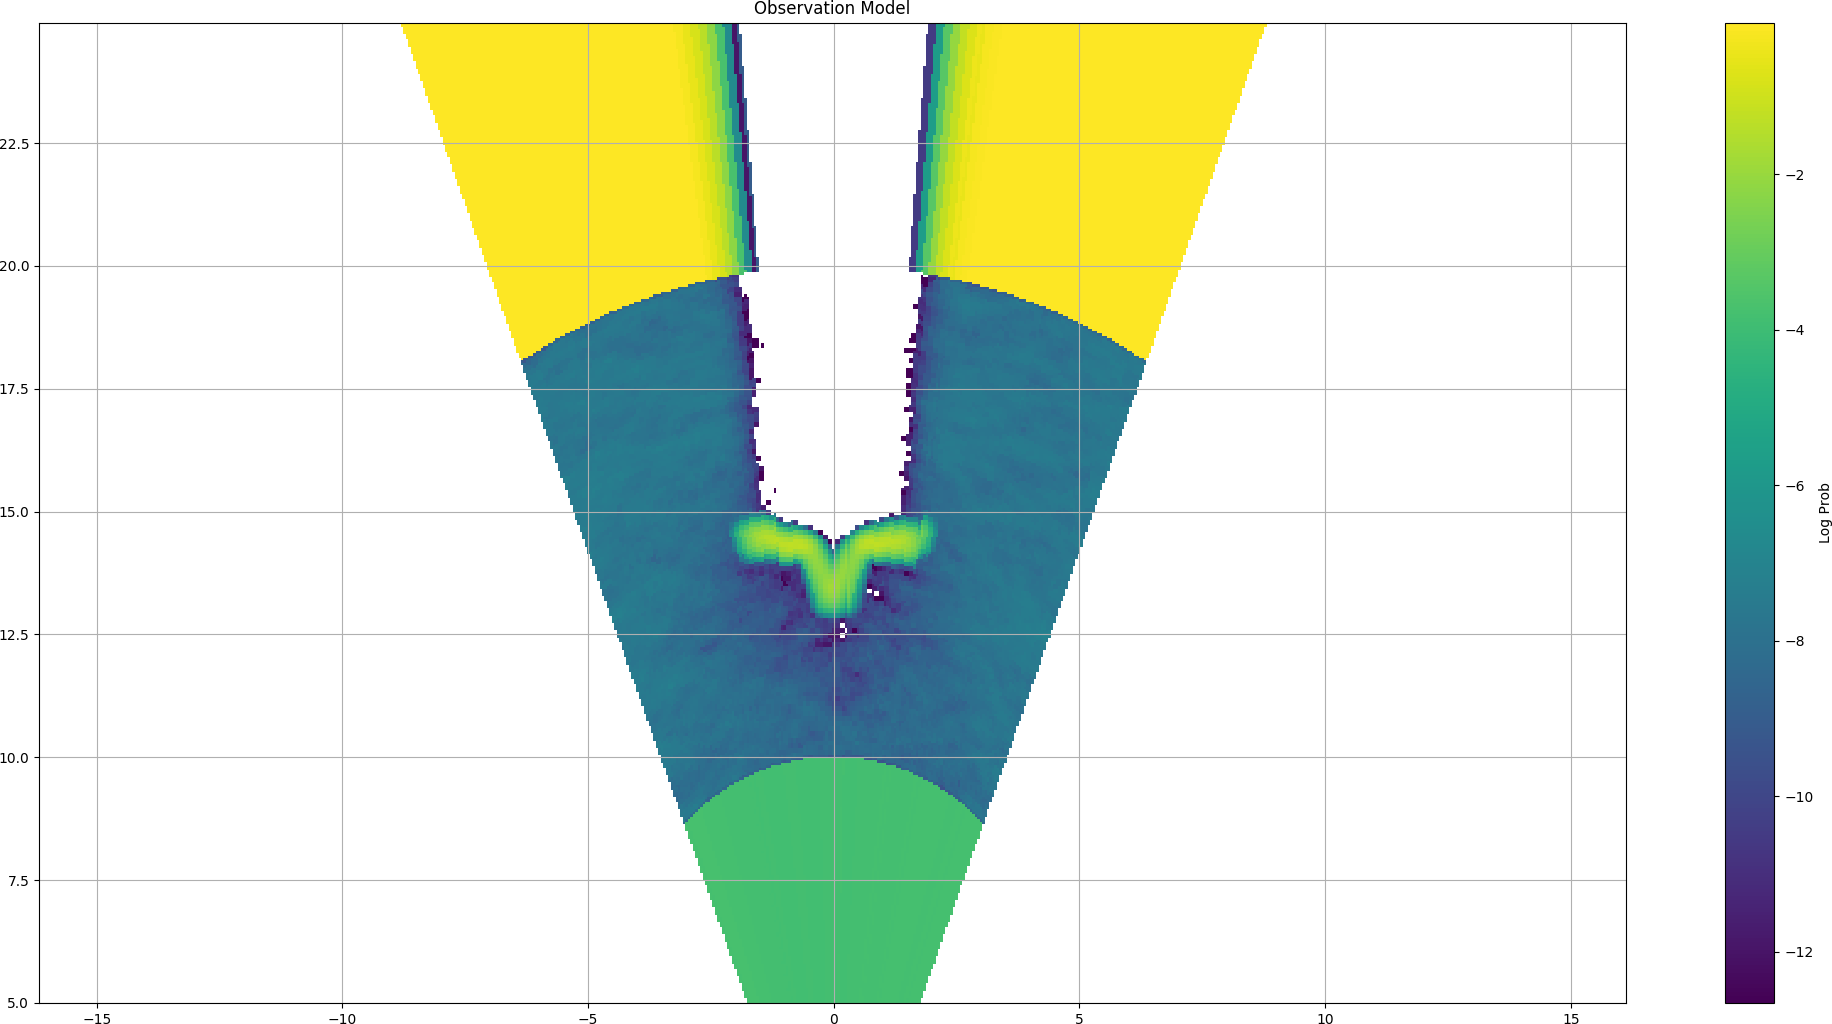
\includegraphics[width=\textwidth]{figures/star_model.png}
  \caption{Simulation. On the left is the simular LIDAR scan of the environment.
    The right figure depicts the ground truth position of all objects in the
    scene.}
  \label{fig:star_model}
\end{figure*}

\begin{figure*}
  \centering
  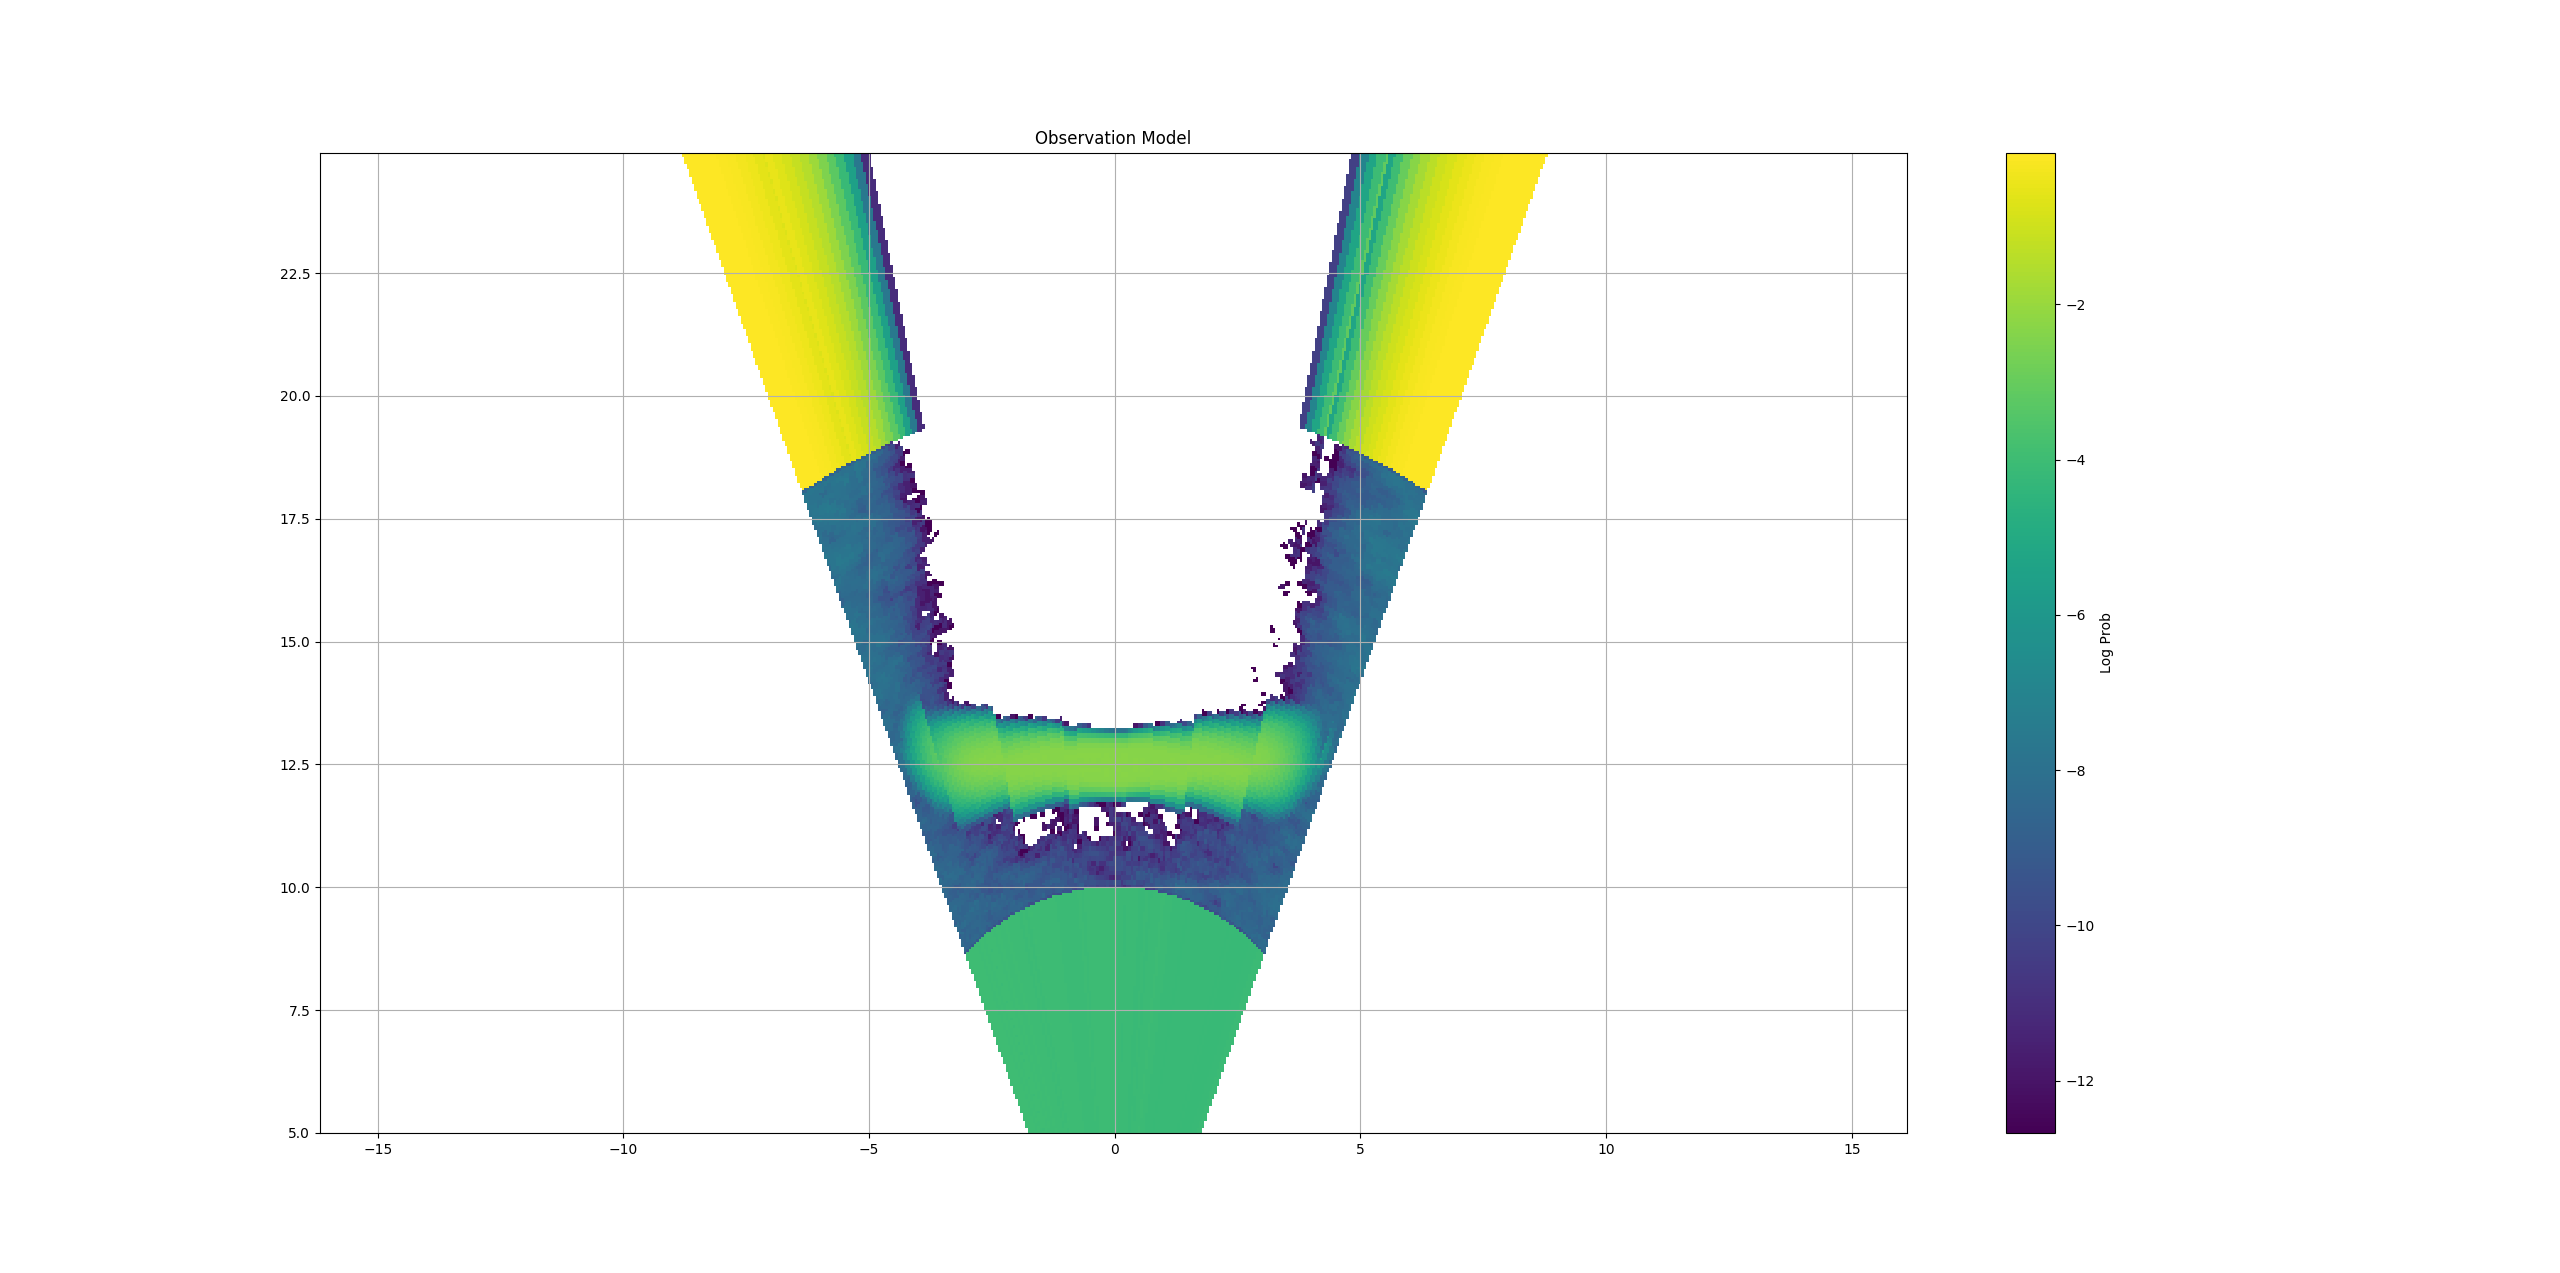
\includegraphics[width=\textwidth]{figures/box_model.png}
  \caption{Simulation. On the left is the simular LIDAR scan of the environment.
    The right figure depicts the ground truth position of all objects in the
    scene.}
  \label{fig:box_model}
\end{figure*}

\section{Detection}

We want to build a map that represents the probability that a object exists at
any particular position $(x, y)$ and orientation $\theta$:
%
\begin{align}
  p(\text{ object at $(x, y)$ and orientation $\theta$ } | \mathbf{Z})
  \text{.}
\end{align}
%
We call this the local map. To build this map for every given $(x, y)$ and
$\theta$, we compute \eqref{eq:detection_prob}. Additionally, we can perform
non-maximal suppression to produce just a list of detections and their positions
and orientations.

\section{Preliminary Results}\label{sec:results}

\subsection{Model Building}

We build models as described in \secref{sec:training}. A few different model
types are shown in \figref{fig:models}.

\begin{figure*}
  \centering
  \begin{subfigure}[]{0.3\linewidth}
    \centering
    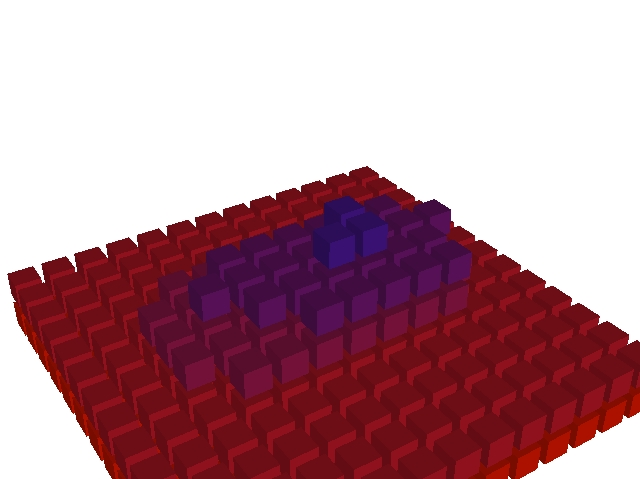
\includegraphics[height=1.5in]{figures/car_marginal.jpg}
    \caption{Na\"ive Bayes (\unit{50}{\cm})}
    \label{fig:nb}
  \end{subfigure}
  \begin{subfigure}[]{0.3\linewidth}
    \centering
    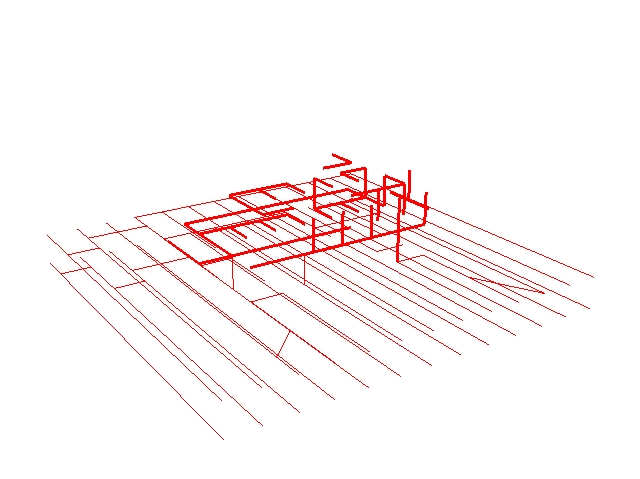
\includegraphics[height=1.5in]{figures/car_tree.jpg}
    %\caption{An example of a \ac{CLT} built for a car. For easier viewing, edges
    %  in the tree that link to nodes that are usually unoccupied are not rendered,
    %  and edges above the ground plane are rendered as thicker lines.}
    \caption{\ac{CLT} (\unit{50}{\cm})}
    \label{fig:clt}
  \end{subfigure}
  \begin{subfigure}[]{0.3\linewidth}
    \centering
    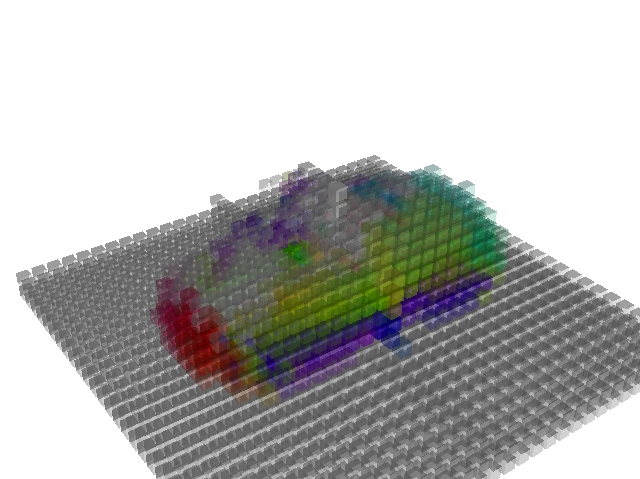
\includegraphics[height=1.5in]{figures/car_fm.jpg}
    \caption{Surface Normals (\unit{20}{\cm})}
    \label{fig:sn}
    %\caption{An example of a model with surface normals. Each voxel is colored by
    %  the most commonly observed surface normal orientation. The hue represents the
    %  surface normal's rotation about the vertical axis, and the saturation
    %  represents the surface normal's angle from the xy plane.}
  \end{subfigure}
  \caption{In \figref{fig:nb}, we see an example of a Na\"ive Bayes model for a
    car. Voxels are colored by z-height, and only voxels that are likely to be
    occupied are rendered. In \figref{fig:clt}, we see the \ac{CLT} as computed
    over the model. Only edges between voxels that are usually occupied are
    shown, with edges above the ground plane rendered as thicker lines. In
    \figref{fig:sn}, we see the model augmented with surface normals. Each voxel
    is colored by the most commonly observed surface normal orientation. The hue
    represents the surface normal's rotation about the vertical axis, and the
    saturation represents the surface normal's angle from the xy plane.}
  \label{fig:models}
\end{figure*}

\subsection{Detection Results}

While demonstrating some promising results (such as those shown in
\figref{fig:badge}, the proposed method still reports a significant number
of false positives. For example, in \figref{fig:ex2} the algorithm is able to
detect the two cars. However, it also believes that the building wall is a car,
due to the fact that it exhibits very similar structural appearance and surface
normals as the side of a car would. In \figref{fig:ex3}, we can see many correct
car detections on the road, but a similar problem occurs with the structure to
either side of the road. These examples were run using the model described in
\secref{sec:normals}, but similar behavior is exhibited with all models
described above.

\begin{figure}[!t]
  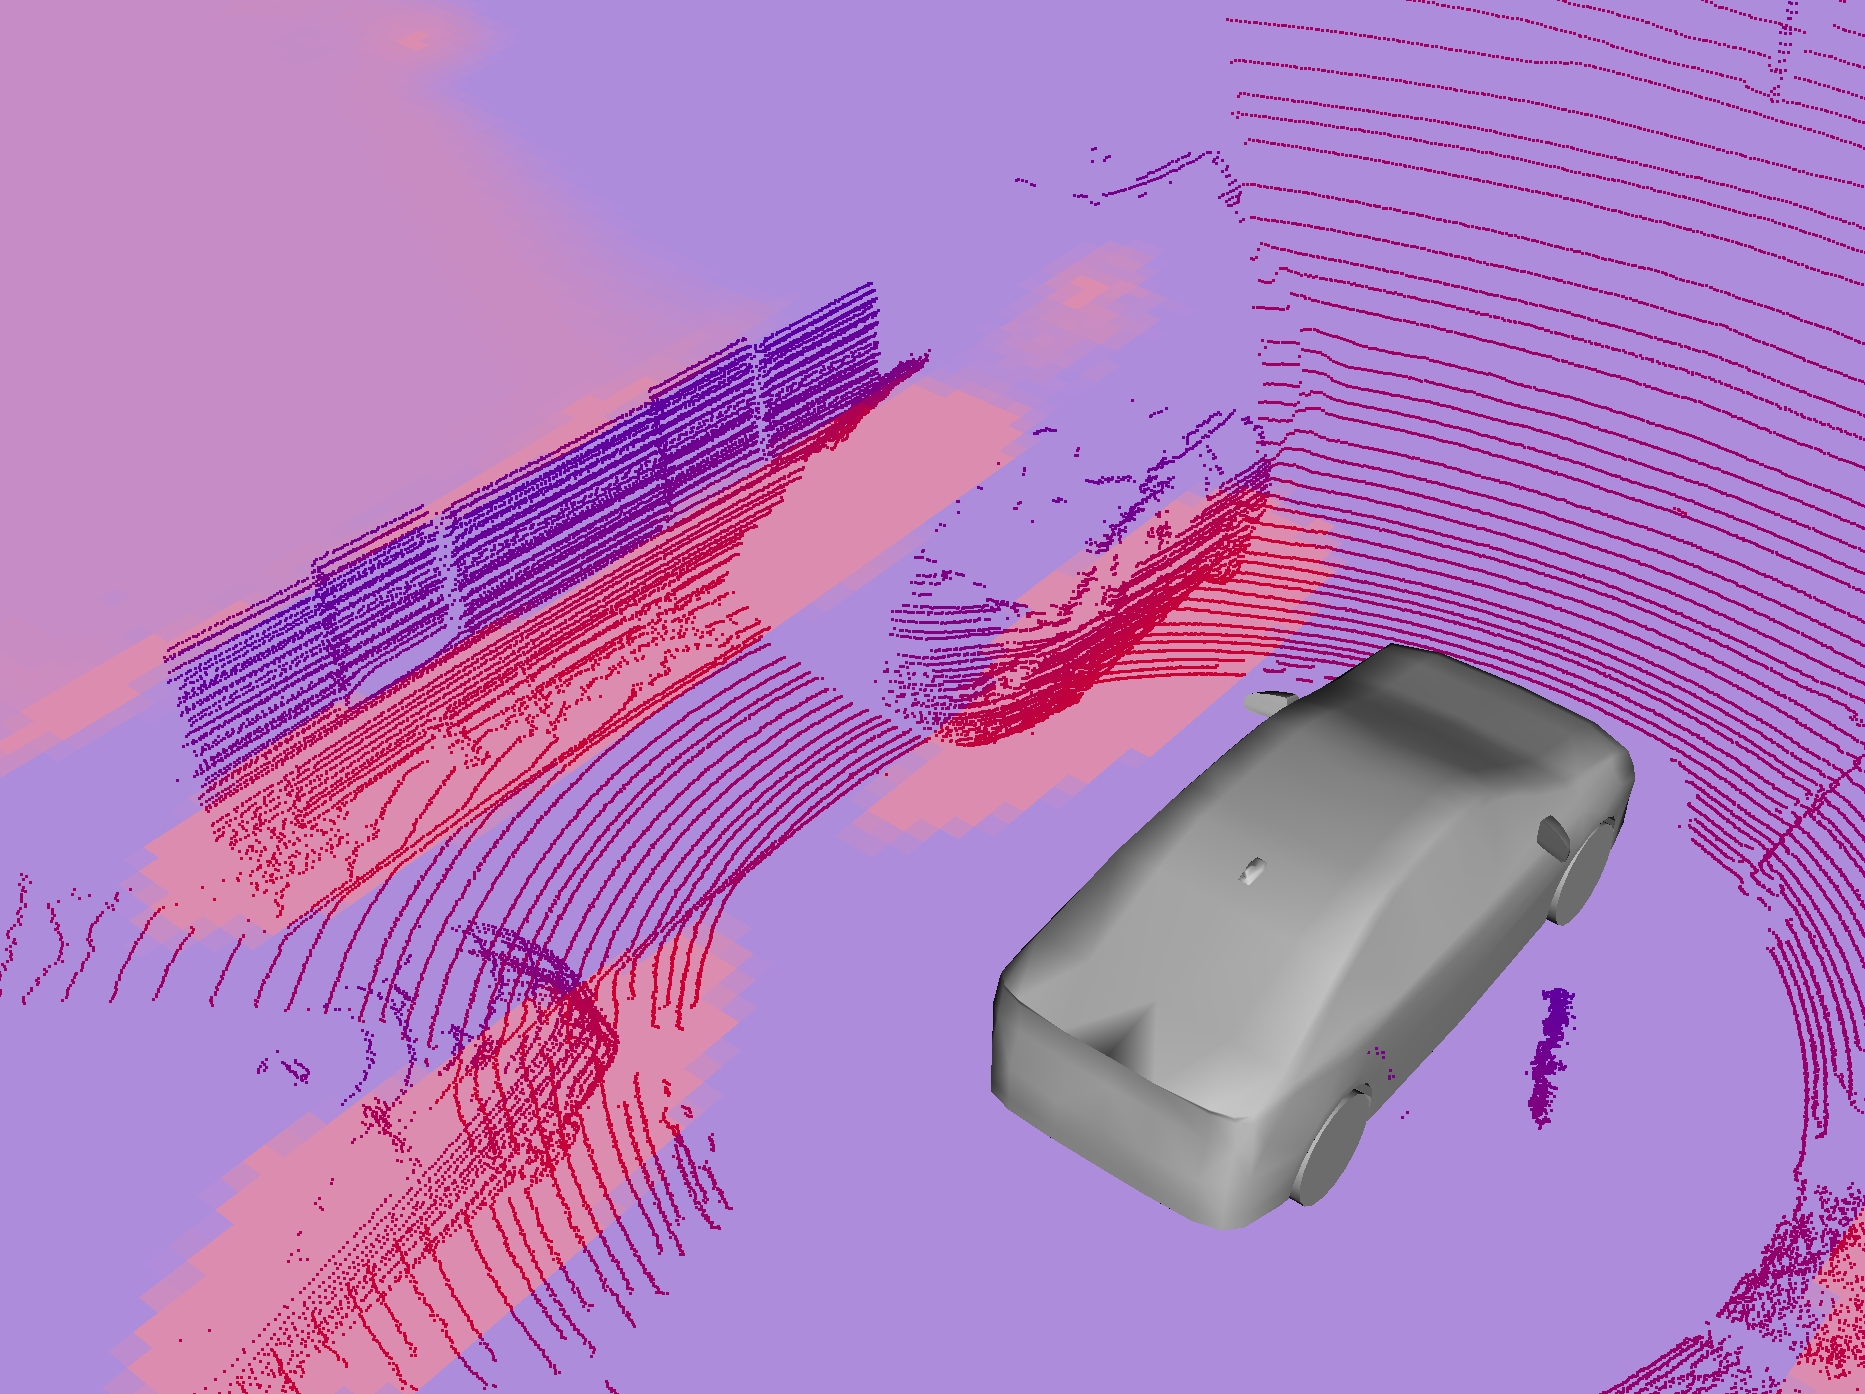
\includegraphics[width=\columnwidth]{figures/ex2.jpg}
  \caption{A very common fault case. Even with surface normals or a joint
    dependency model, often background such as building walls are supported by
    the car's  observation model. Car likelihoods are shown in red.}
  \label{fig:ex2}
\end{figure}

\begin{figure}[!t]
  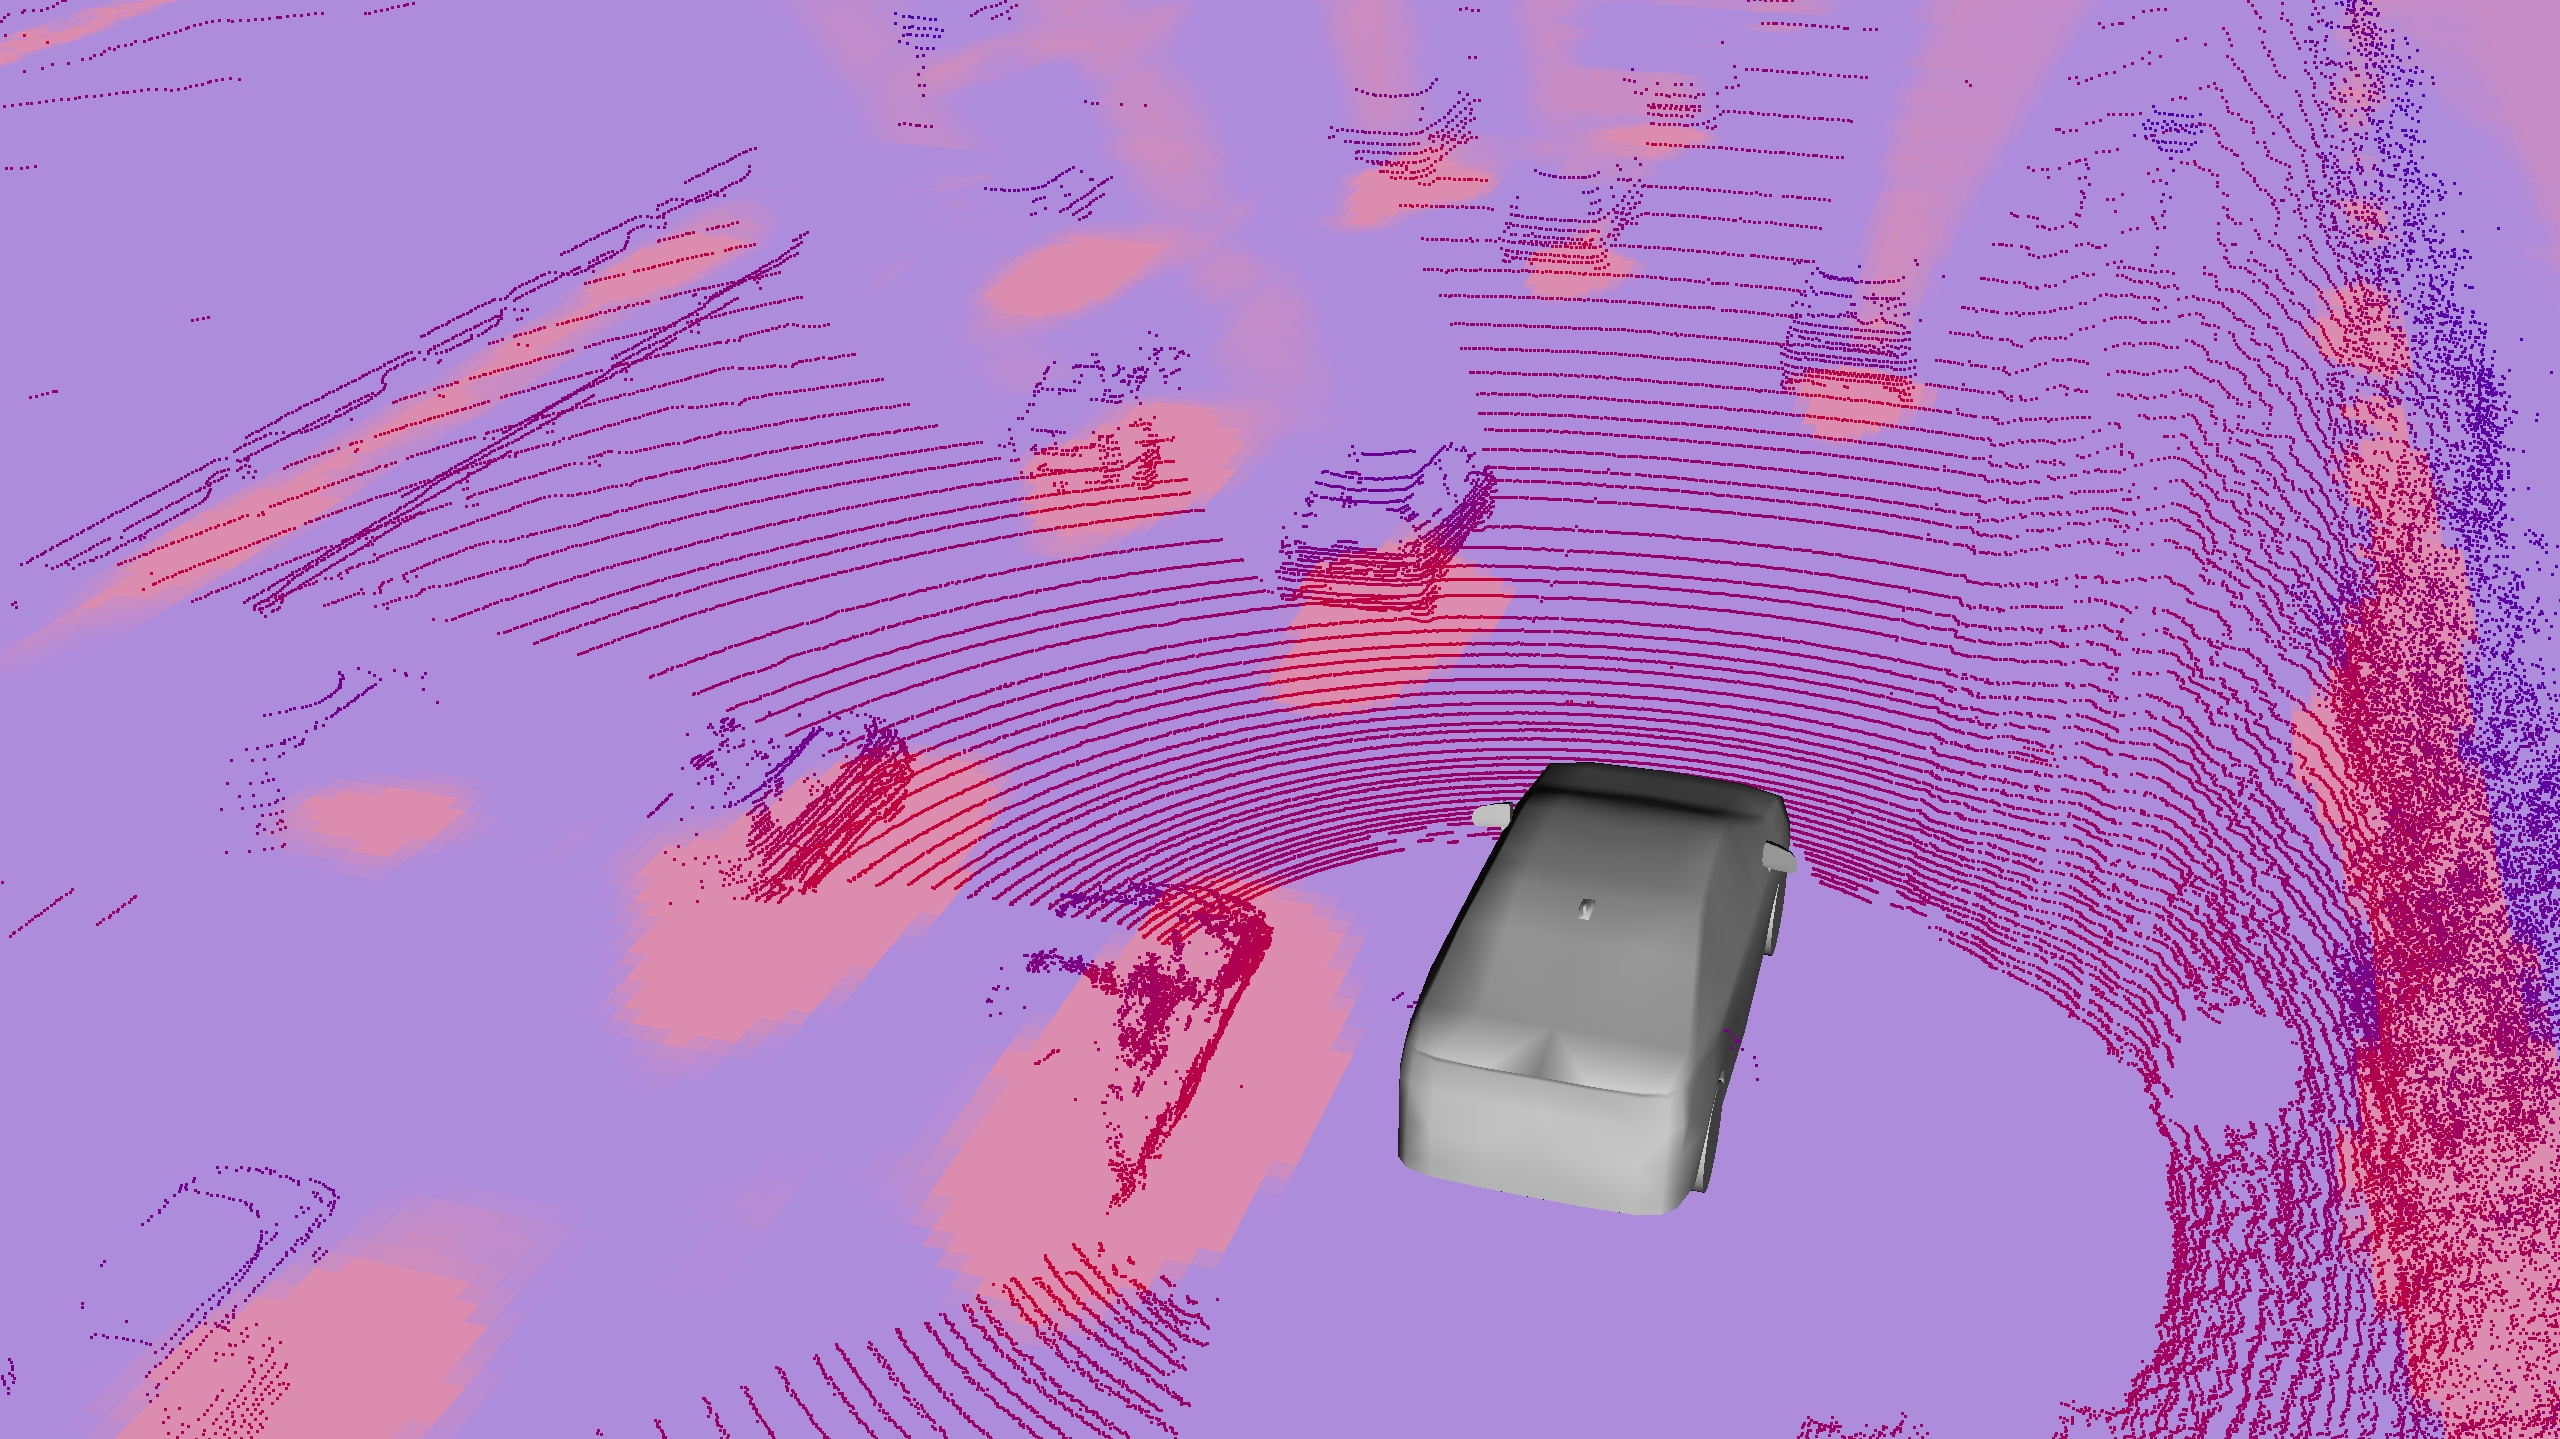
\includegraphics[width=\columnwidth]{figures/ex3.jpg}
  \caption{An example with both good detections and false positives on the
    background structure on either side of the road. Car likelihoods are shown
    in red.}
  \label{fig:ex3}
\end{figure}


%\begin{abstract}
%
Estimating the pose of visible and occluded objects in the environment is a core
competency for autonomous robotic systems. Standard object detection pipelines
typically report a list of object locations per class, but do not directly
support reasoning about where objects \emph{could} be. In this work, we work
towards augmenting the state-of-the-art LIDAR detection algorithms with a notion
of free and unknown space. Importantly, this distinction enables computing a
distribution over per class object locations, which allows reasoning about
anywhere in the immediate environment, including into occluded regions. We
show some preliminary results on the publicly available KITTI dataset.
%
\end{abstract}

%\acresetall

%\IEEEpeerreviewmaketitle

%\acused{GPU}

%\section{Introduction}\label{sec:intro}

A core competency of many autonomous systems is to be aware of the state of
their environments so that they may operate safely in them. For example, an
autonomous vehicle needs to be aware of other cars on the road for a path
planning module to propose safe actions. This object detection task has been
extensively studied in the literature using different sensor modalities,
including camera imagery and \ac{LIDAR}.

However, object detection alone does not paint a complete picture of the
environment for the robot. It is also critical for a robot to make inferences
and decisions regarding where objects possibly \emph{could} be; for example, a
robot might need to ask ``how likely is it that a pedestrian is present in this
occluded region?" The answer to this question can be the difference between
driving through an intersection unhindered or cautiously anticipating a
pedestrian hidden behind a parked car.

\figref{fig:badge} shows an example of a situation that an autonomous car might
encounter. In addition to detecting the cars present in the environment, we
wish to capture areas we know are absent of cars (shown in blue) or areas where
there might be cars that are hidden (such as the occluded region in the top
right).

The state-of-the-art in object detection, while performing very well in the pure
detection task, is ill-suited to answer these types of queries. These methods
typically do not fully model the nature of range-based sensors such as
\ac{LIDAR}, often using solely the points that are returned. Thus, there is no
way to differentiate between free and unknown regions of the world.

Occupancy mapping and related work is better suited for differentiating between
free and unknown space, as they explicitly model these. However, this mapping is
typically performed per voxel, and there is no notion of the potential absence
or presence of an \emph{object class}.

In this paper, we blend these two paradigms; we present a method that
consumes \ac{LIDAR} data and produces a probabilistic distribution of object-level
detections that can represent known objects in the world, areas were objects are
known to be absent, and regions of uncertainty. To achieve this, we rely on
techniques from both approaches, including ray-casting to sweep out free space
and the use of object-level observation models. Additionally, we formulate our
approach in a Bayesian framework, allowing for simple integration of additional
sensor modalities.

The goals of this work include:
%
\begin{itemize}
  \item Explicitly modeling occupied, free, and unknown space in a Bayesian
    formulation that is easily amendable to multi-modal sensing or temporal
    updates.
  \item Generation of a probabilistic detection map that can be queried at any
    location for the presence of a given object.
\end{itemize}
%
Additionally, we evaluate this approach on the KITTI dataset
\cite{Geiger2013IJRR}.
%
\begin{figure}[!t]
  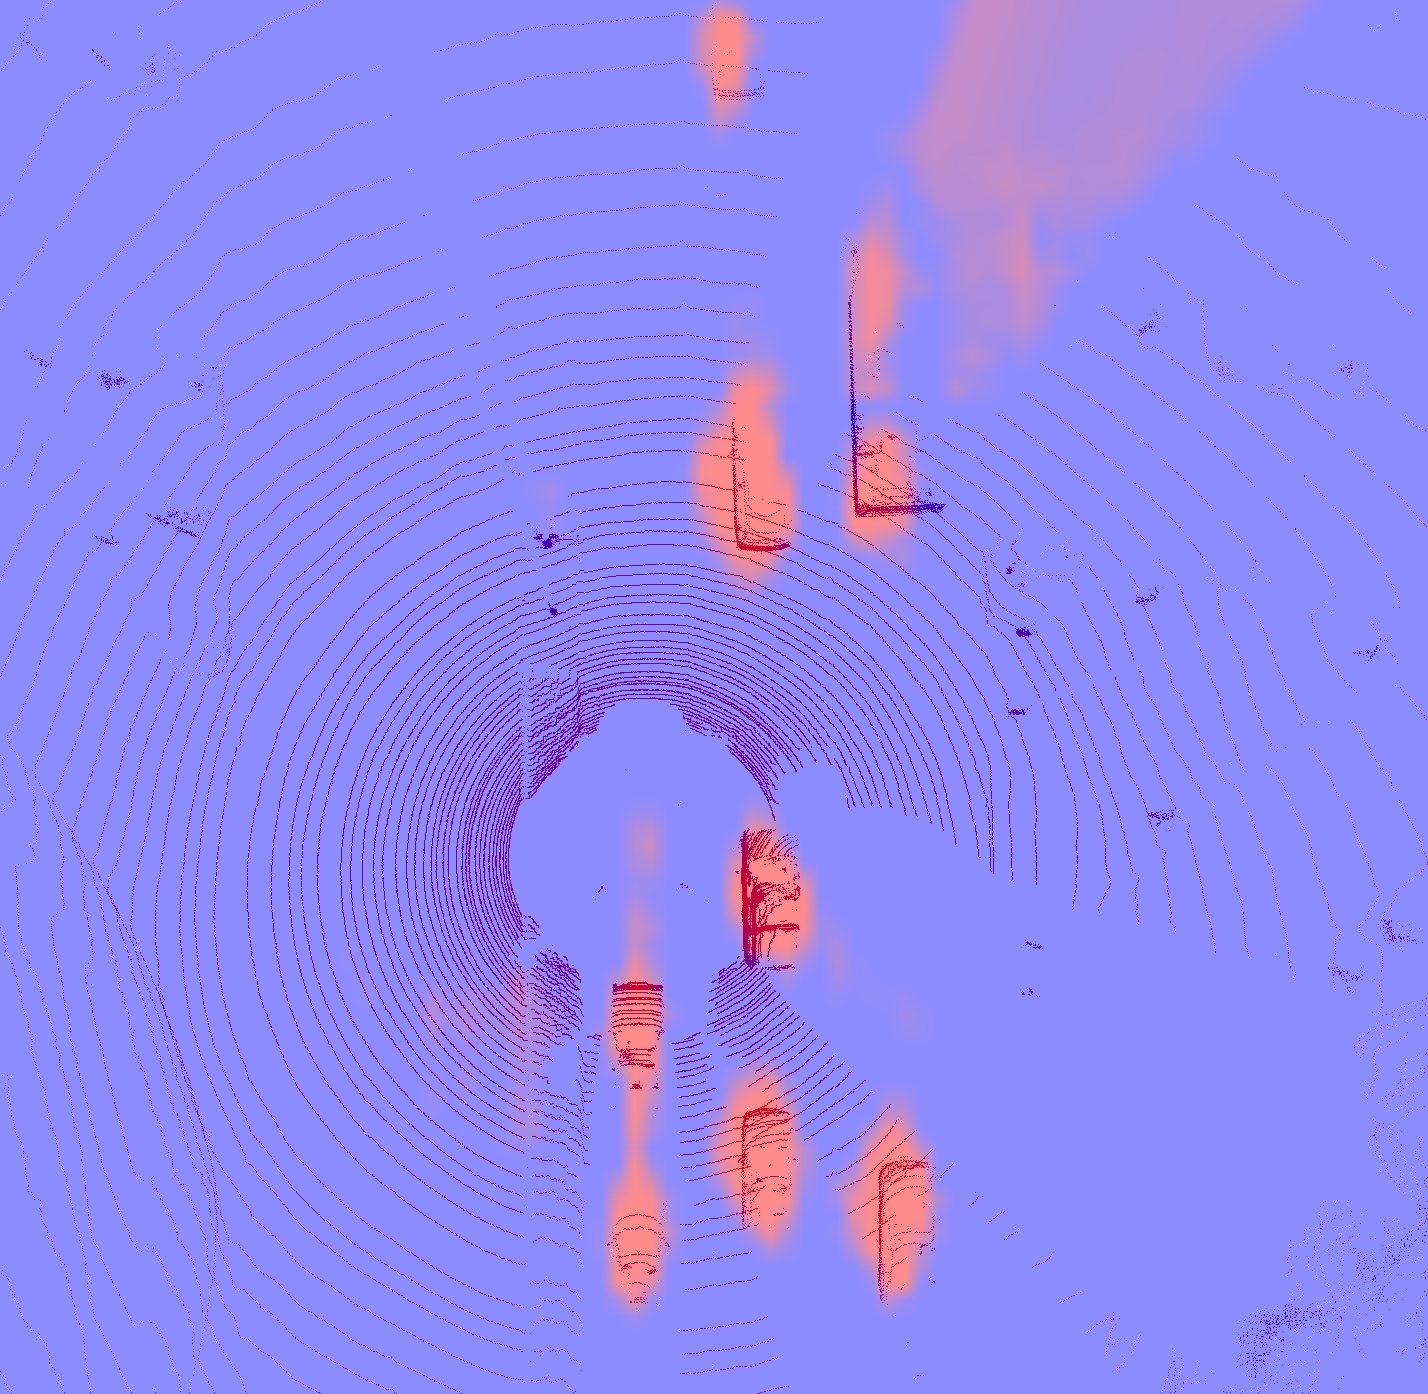
\includegraphics[width=\columnwidth]{figures/badge2.png}
  \caption{\aku{Placeholder badge figure, make a better version}. A bird's eye
    view of sample output from our proposed system run on the KITTI dataset. Red colors indicate high
    probabilities for cars, blue indicates high probabilities for background.
    (Best viewed in color.) }
  \label{fig:badge}
\end{figure}

%\section{Related Work}\label{sec:rw}

There is a rich literature in both object-level detection and probabilistic
mapping. In object detection, many methods can be regarded as simply taking some
kind of object classifier and applying it to locations in the environment. These
locations can either be searched exhaustively or by some guided method, such as
segmentation or region proposal. \citet{wang2012could} segmented and clustered a
laser scan before classifying each segment according to background or foreground
object. \citet{wang2015RSS} implemented a sliding window SVM detector with a
voting scheme that allowed for efficient processing of sparse \ac{LIDAR} data.
Building upon this idea, \citet{Engelcke2017ICRA} showed that this same voting
scheme could be adapted for use with a \ac{CNN}.

Another approach is to process all of the sensor data together. In one of the
earlier works, \citet{petrovskaya-2009} created virtual 2D scans from \ac{LIDAR}
data and used a Bayes filter per object to estimate both the dynamics and simple
geometries properties, such as width and length. This filter is then maintained
over time as more observations are made. More recently, this type of approach has
been popular in a deep learning approach using camera data
\citep{yang2016exploit, deepmanta_cvpr17, Ren17CVPR}, but has also been applied
to \ac{LIDAR} sensor data as well. \citet{Li2016RSS} process a range image from
a \ac{LIDAR} sensor using a \ac{FCN} to generate bounding boxes for car
detections. \citet{Chen2017CVPR} build a fusion network that takes as input both
camera imagery and also multiple views of a \ac{LIDAR} point cloud, such as a
bird's eye view or a front view. However, these approaches do not explicitly model
the notion of free space and occluded regions.

Occupancy mapping \cite{thrun2005probabilistic} and its derivatives (such as
\cite{hornung13auro}) are commonly used to model the full
information captured by a range sensor such as \ac{LIDAR}, properly modeling
free and occluded space while also representing unknown areas at the level of discrete
voxels. \citet{gpmaps_ijrr12} introduced Gaussian process occupancy maps, a
technique that exploits the structure of environments (e.g., the occupancy of
some position in the world is correlated with its neighborhood). More recently,
\citet{Ramos-RSS-15} introduced Hilbert mapping, a somewhat related approach in
which a kernelized logistic regression is trained to predict occupied or free
space from online sensor measurements. Extensions of this framework explored how
to leverage the choice of kernels used in the regression, essentially modeling
features that capture structure primitives \citep{Guizilini-RSS-17,
  guizilini2016large}. However, these approaches do not focus on capturing
specific object classes.

Recently, there has been some work in object detection and classification from
occupancy grids or similar representations, typically using some kind of
volumetric or multiview \ac{CNN} \cite{qi2016volumetric, maturana2015voxnet}.
These methods tend to do well with occlusions, as evidenced by the
performance of similar techniques in shape completion \cite{smith2017CORL,
  dai2017complete}. However, these approaches focus on classify a single
instances of an object from a single occupancy grid or similar representation.
As such, it is intractable to scale them into an exhaustive search.

Our work lies at the intersection of object detection and occupancy mapping. We
propose a representation that provides the benefits of both approaches, namely,
understanding at an object level and capturing both known and unknown areas.


%\section{Detection Likelihood Map}\label{sec:dlm}

Our goal is to compute a detection map that captures how likely it is for an
object to exist at a particular location in the world. As our work is targeted
for applications with autonomous vehicles, for runtime performance, we make the
assumption that the world is 2.5D. Namely, we assume that all objects exist on a
horizontal plane and their pose can be fully described by their 2D location and
rotation. However, we fully model the 3D nature of the sensor observations.

We receive a set of \ac{LIDAR} observations, $\mathbf{Z} = \{z_{1:n_z}\}$. Given
these, we evaluate:
%
\begin{align}
  p(\mathrm{obj_{c, x}}| \mathbf{Z}) \text{,} \label{eq:detection_map}
\end{align}
%
where $\mathrm{obj_{c, x}}$ denotes the presence of an object of class $c$ with
pose $x$. As we focus on KITTI, the classes we are concerned with are Car,
Pedestrian, and Cyclist. Additionally, we model a Background class as well. We
refer to \eqref{eq:detection_map} as a probabilistic detection map. Our goal is
to evaluate and generate this map.

Applying Bayes' rule, we have:
%
\begin{align}
  p(\mathrm{obj_{c, x}} | \mathbf{v}) &=
    \frac
      {p(\mathrm{obj_{c, x}}) p(\mathbf{Z} | \mathrm{obj_{c, x}})}
      {p(\mathbf{Z})}
  \text{,}
  \label{eq:bayes}
\end{align}
%
where $p(\mathrm{obj_{c, x}})$ is an object prior,
$p(\mathbf{Z} | \mathrm{obj_{c, x}})$ is the observation model, and
$p(\mathbf{Z})$ is a normalization factor.

The key part of \eqref{eq:bayes} is the observation model. We require an
observation model that is expressive enough to detect objects and differentiate
between different classes. At the same time, we must be able to evaluate this
model quickly for different classes and poses so that it is tractable to
evaluate \eqref{eq:bayes} for a large number of object poses and classes to
fully build the detection map.

%\section{Method} \label{sec:method}

We investigate several different ways to evaluate the observation model.

\subsection{Ray-Based}

In \cite{ushani_raybased}, we extensively studied how to evaluate the
observation by using a ray-based approach. Each observation $z_i$ is modeled as
a ray from the sensor origin to the point return (thus capturing the free space
between the sensor and the returned point). We built a ray-based observation
model for each object class using a discretized lookup table of histograms that
were learned during training. Additionally, to improve performance when dealing
with multiple classes, the conditional dependence of $z_i$ on $z_{i-1}$ was
modeled as well. While this approach showed promising results in a 2D simulated
world, it was intractable to scale up to 3D, with the chief problem being
training a higher dimensional observation model.

\subsection{Occupancy Grid}

To make the problem more tractable in 3D, we considered building an occupancy
grid from the \ac{LIDAR} observations $\mathbf{Z}$. This occupancy grid consists
of a sparse set of voxels $\mathbf{V} = \{v_{1:n_v}\}$, where each voxel $v_i$
is labeled as either free or occupied. Any voxels not contained in this sparse
set is considered to be unknown. We compute $\mathbf{V}$ by performing
ray-casting using Bresenham's ray tracing algorithm
\cite{bresenham1965algorithm}. This can be efficiently implemented on a \ac{GPU}

Thus, for our observation model, we now wish to evaluate:
%
\begin{align}
  p(\mathbf{V} | \mathrm{obj_{c, x}}) \text{.} \label{eq:detection_map}
\end{align}

\subsubsection{Na\"ive Bayes} \label{sec:naive_bayes}

One approach is to make the independence assumption:
%
\begin{align}
  p(\mathbf{V} | \mathrm{obj_{c, x}}) &= \prod_i p(v_i | \mathrm{obj_{c, x}})
  \text{.}
\end{align}
%
The key advantage of this approach is its simplicity and speed.
However, we find that this assumption leads to significant confusion between
classes. As each voxel is assumed to be independent given the presence of an
object, this model does not capture any of the dependencies between voxels in
the case in intra-class variation, leading to degradation in performance. For
example, this model cannot easily distinguish between a car and a bush that is
roughly the same size as a car.

\subsubsection{Chow-Liu Tree Model} \label{sec:clt}

Similar to our work in \cite{ushani_raybased}, we propose approximating the full
joint distribution $p(\mathbf{V} | \mathrm{obj_{c,x}})$ by approximating a
\ac{CLT} \citep{chow1968approximating}.

For the observations $\mathbf{V} = \{v_1, \ldots, v_{n_z}\}$, a \ac{CLT} finds a
first order dependency tree between them that minimizes the \ac{KLD} between the
approximated distribution $P$ and the true full joint distribution $Q$:
%
\begin{align}
  D(P || Q) &= -\sum I(v_i, v_{p(i)}) + \sum H(v_i) - H(\mathbf{V})
  \label{eq:kld}
  \text{,}
\end{align}
%
where $I(v_i, v_{p(i)})$ is the mutual information between $v_i$ and its parent
in the tree $v_{p(i)}$, $H(v_i)$ is the entropy of $v_i$, and $H(\mathbf{V})$ is
the joint entropy of $\{v_1, \ldots, v_{n_z}\}$. To minimize the \ac{KLD}, the
\ac{CLT} finds the spanning tree amongst $\mathbf{V}$ that maximizes the total
pairwise mutual information, as the latter two terms in \eqref{eq:kld} are
independent of the dependency tree's structure.

To evaluate the \ac{CLT} approximation of the distribution, we compute:
%
\begin{align}
  p(\mathbf{V)} &\approx p_{clt}(\mathbf{V}) = p(v_r) \prod p(v_i | v_{p(i)})
\end{align}
%
where $v_r$ is the voxel chosen as the root of the spanning tree.

\subsubsection{Greedy CLT Approximation} \label{sec:greedy_clt}

The \ac{CLT} does better at approximating the true distribution than the na\"ive
approach. However, it can prove costly to use at runtime. Since the set of
voxels $\mathbf{V}$ is continually changing, we cannot simply build the \ac{CLT}
offline to evaluate at runtime. We could rebuild the \ac{CLT} every time we need
to use it, but that requires solving the maximum spanning tree for each
evaluation and would still prove costly. Updating the \ac{CLT} or marginalizing
out voxels that are unobserved quickly becomes intractable as well.

We can comprise between approximating the joint distribution and runtime by
taking a greedy approach. Consider some some of voxel observations $\mathbf{V}$
that we wish to evaluate. We choose the first $v_1$ to be the root of the tree.
Next, for every following $v_i$ we find the preceding voxel observation $v_j, j
< i$ that maximizes $I(v_i, v_j)$ and add this edge to the tree. As voxels tend
to have more mutual information with other voxels that are nearby, we can
further save on runtime by only searching for $j > i - n_v$, where $n_v$ is a
constant, where we take care to process $\mathbf{V}$ in spatial order.

\subsubsection{Surface Normals} \label{sec:normals}

We can augment the occupancy grid by computing surface normals. For any voxel
$v_i$ that is occupied and thus contains some \ac{LIDAR} points $\{z_j\}$, we
can approximate the surface captured by these points and compute a surface
normal. We do this by computing the covariance $\mat{C}$ of all points within
$v$ and finding the eigenvector of $\mat{C}$ corresponding to the smallest
eigenvector. These surface normals can then be used to augment
any of the above approaches, although we specifically considered it with
\secref{sec:naive_bayes}. For example, instead of evaluating just
%
\begin{align}
  p(v_i \text{ is occupied } | \mathrm{obj_{c,x}}) \text{,}
\end{align}
%
as we would in \secref{sec:naive_bayes}, we now evaluate
%
\begin{align}
  p(v_i \text{ is occupied } | \mathrm{obj_{c,x}}) p(v_i \text{ has normal } \vec{n}
  | \mathrm{obj_{c, x}}) \text{.}
\end{align}

\subsection{Training}

All of our models were trained using KITTI data. During the training phase, we
sample observations (i.e., a local occupancy grid) for each class. Once all samples are
extracted, they are then accumulated together to estimate the observation model
for each class. This includes marginal probabilities for
\secref{sec:naive_bayes}, mutual information and conditional probabilities for
\secref{sec:clt} and \secref{sec:greedy_clt}, and discretizied surface normals
for \secref{sec:normals}.

In this work, the model for each object extends extends \unit{6}{\m} in each of $x$ and $y$
and \unit{4}{\m} vertically. A unique model for each is learned for each of 8
orientations from \unit{0} to \unit{360}{\deg}. To compensate for the pose
discretization, we randomly sample several slightly translated and rotated
instances of each object.

%\section{Preliminary Results}\label{sec:results}

\subsection{Model Building}

We build models as described in \secref{sec:training}. A few different model
types are shown in \figref{fig:models}.

\begin{figure*}
  \centering
  \begin{subfigure}[]{0.3\linewidth}
    \centering
    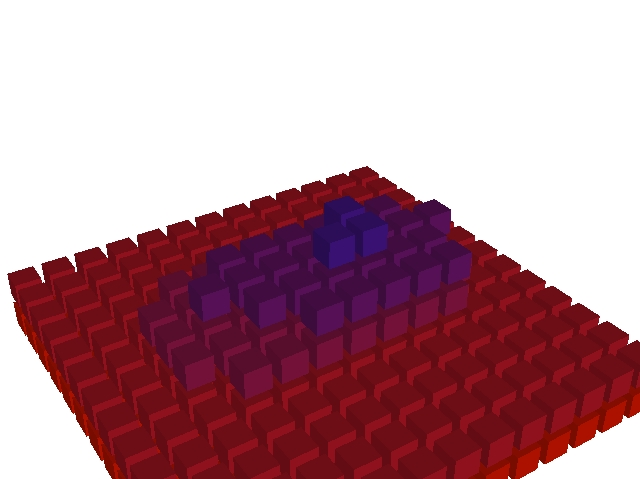
\includegraphics[height=1.5in]{figures/car_marginal.jpg}
    \caption{Na\"ive Bayes (\unit{50}{\cm})}
    \label{fig:nb}
  \end{subfigure}
  \begin{subfigure}[]{0.3\linewidth}
    \centering
    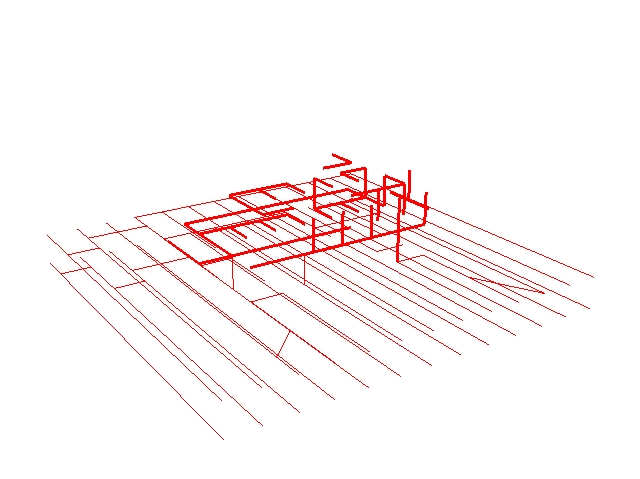
\includegraphics[height=1.5in]{figures/car_tree.jpg}
    %\caption{An example of a \ac{CLT} built for a car. For easier viewing, edges
    %  in the tree that link to nodes that are usually unoccupied are not rendered,
    %  and edges above the ground plane are rendered as thicker lines.}
    \caption{\ac{CLT} (\unit{50}{\cm})}
    \label{fig:clt}
  \end{subfigure}
  \begin{subfigure}[]{0.3\linewidth}
    \centering
    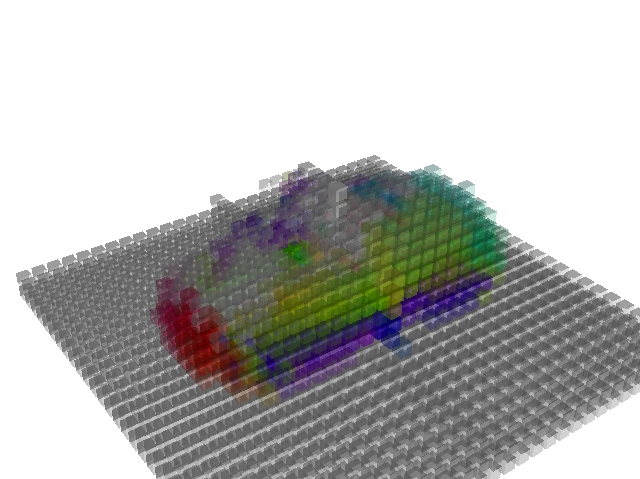
\includegraphics[height=1.5in]{figures/car_fm.jpg}
    \caption{Surface Normals (\unit{20}{\cm})}
    \label{fig:sn}
    %\caption{An example of a model with surface normals. Each voxel is colored by
    %  the most commonly observed surface normal orientation. The hue represents the
    %  surface normal's rotation about the vertical axis, and the saturation
    %  represents the surface normal's angle from the xy plane.}
  \end{subfigure}
  \caption{In \figref{fig:nb}, we see an example of a Na\"ive Bayes model for a
    car. Voxels are colored by z-height, and only voxels that are likely to be
    occupied are rendered. In \figref{fig:clt}, we see the \ac{CLT} as computed
    over the model. Only edges between voxels that are usually occupied are
    shown, with edges above the ground plane rendered as thicker lines. In
    \figref{fig:sn}, we see the model augmented with surface normals. Each voxel
    is colored by the most commonly observed surface normal orientation. The hue
    represents the surface normal's rotation about the vertical axis, and the
    saturation represents the surface normal's angle from the xy plane.}
  \label{fig:models}
\end{figure*}

\subsection{Detection Results}

While demonstrating some promising results (such as those shown in
\figref{fig:badge}, the proposed method still reports a significant number
of false positives. For example, in \figref{fig:ex2} the algorithm is able to
detect the two cars. However, it also believes that the building wall is a car,
due to the fact that it exhibits very similar structural appearance and surface
normals as the side of a car would. In \figref{fig:ex3}, we can see many correct
car detections on the road, but a similar problem occurs with the structure to
either side of the road. These examples were run using the model described in
\secref{sec:normals}, but similar behavior is exhibited with all models
described above.

\begin{figure}[!t]
  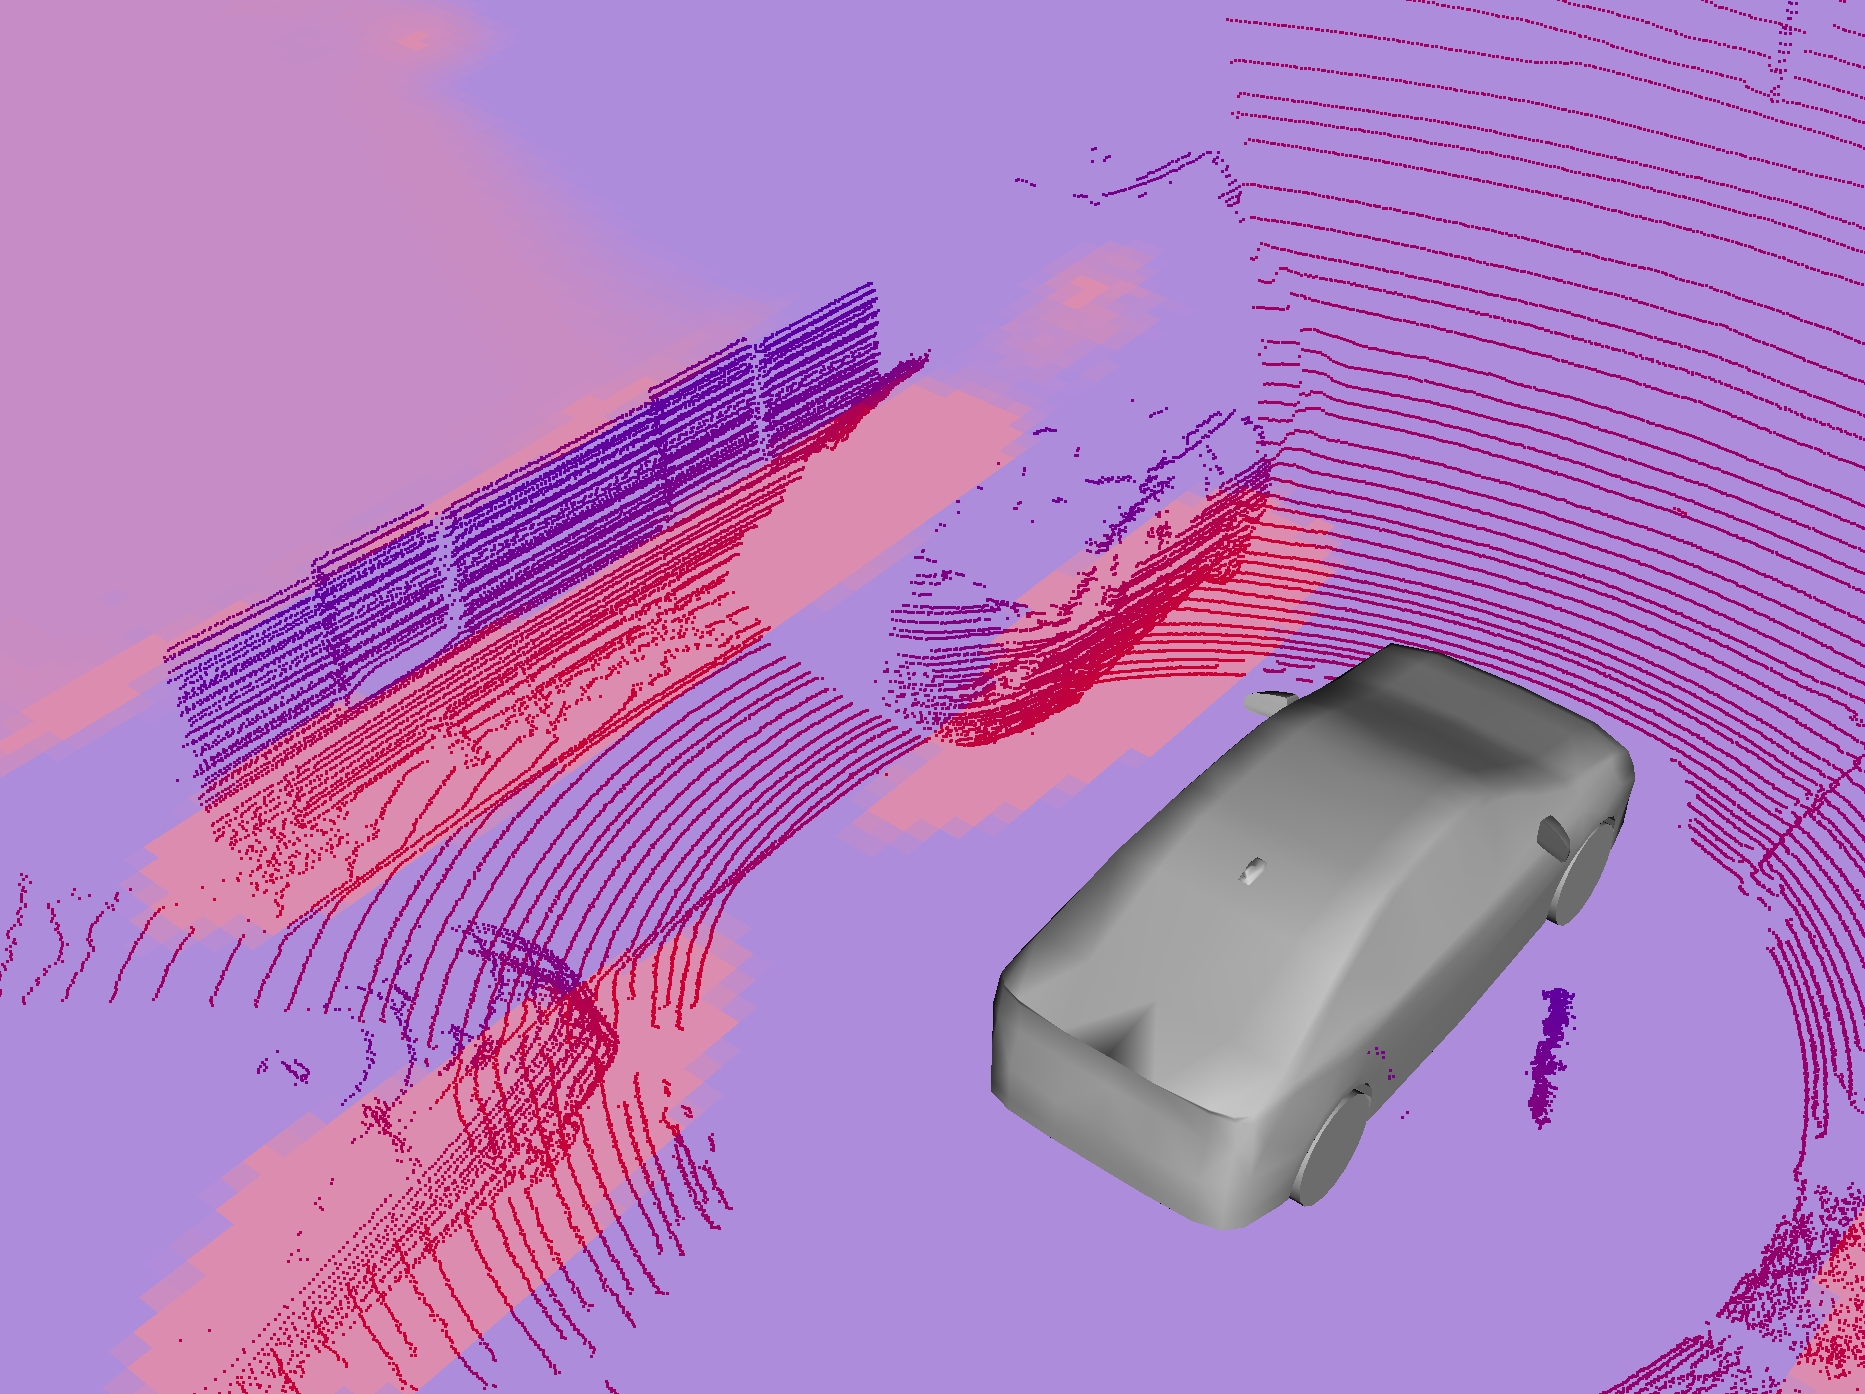
\includegraphics[width=\columnwidth]{figures/ex2.jpg}
  \caption{A very common fault case. Even with surface normals or a joint
    dependency model, often background such as building walls are supported by
    the car's  observation model. Car likelihoods are shown in red.}
  \label{fig:ex2}
\end{figure}

\begin{figure}[!t]
  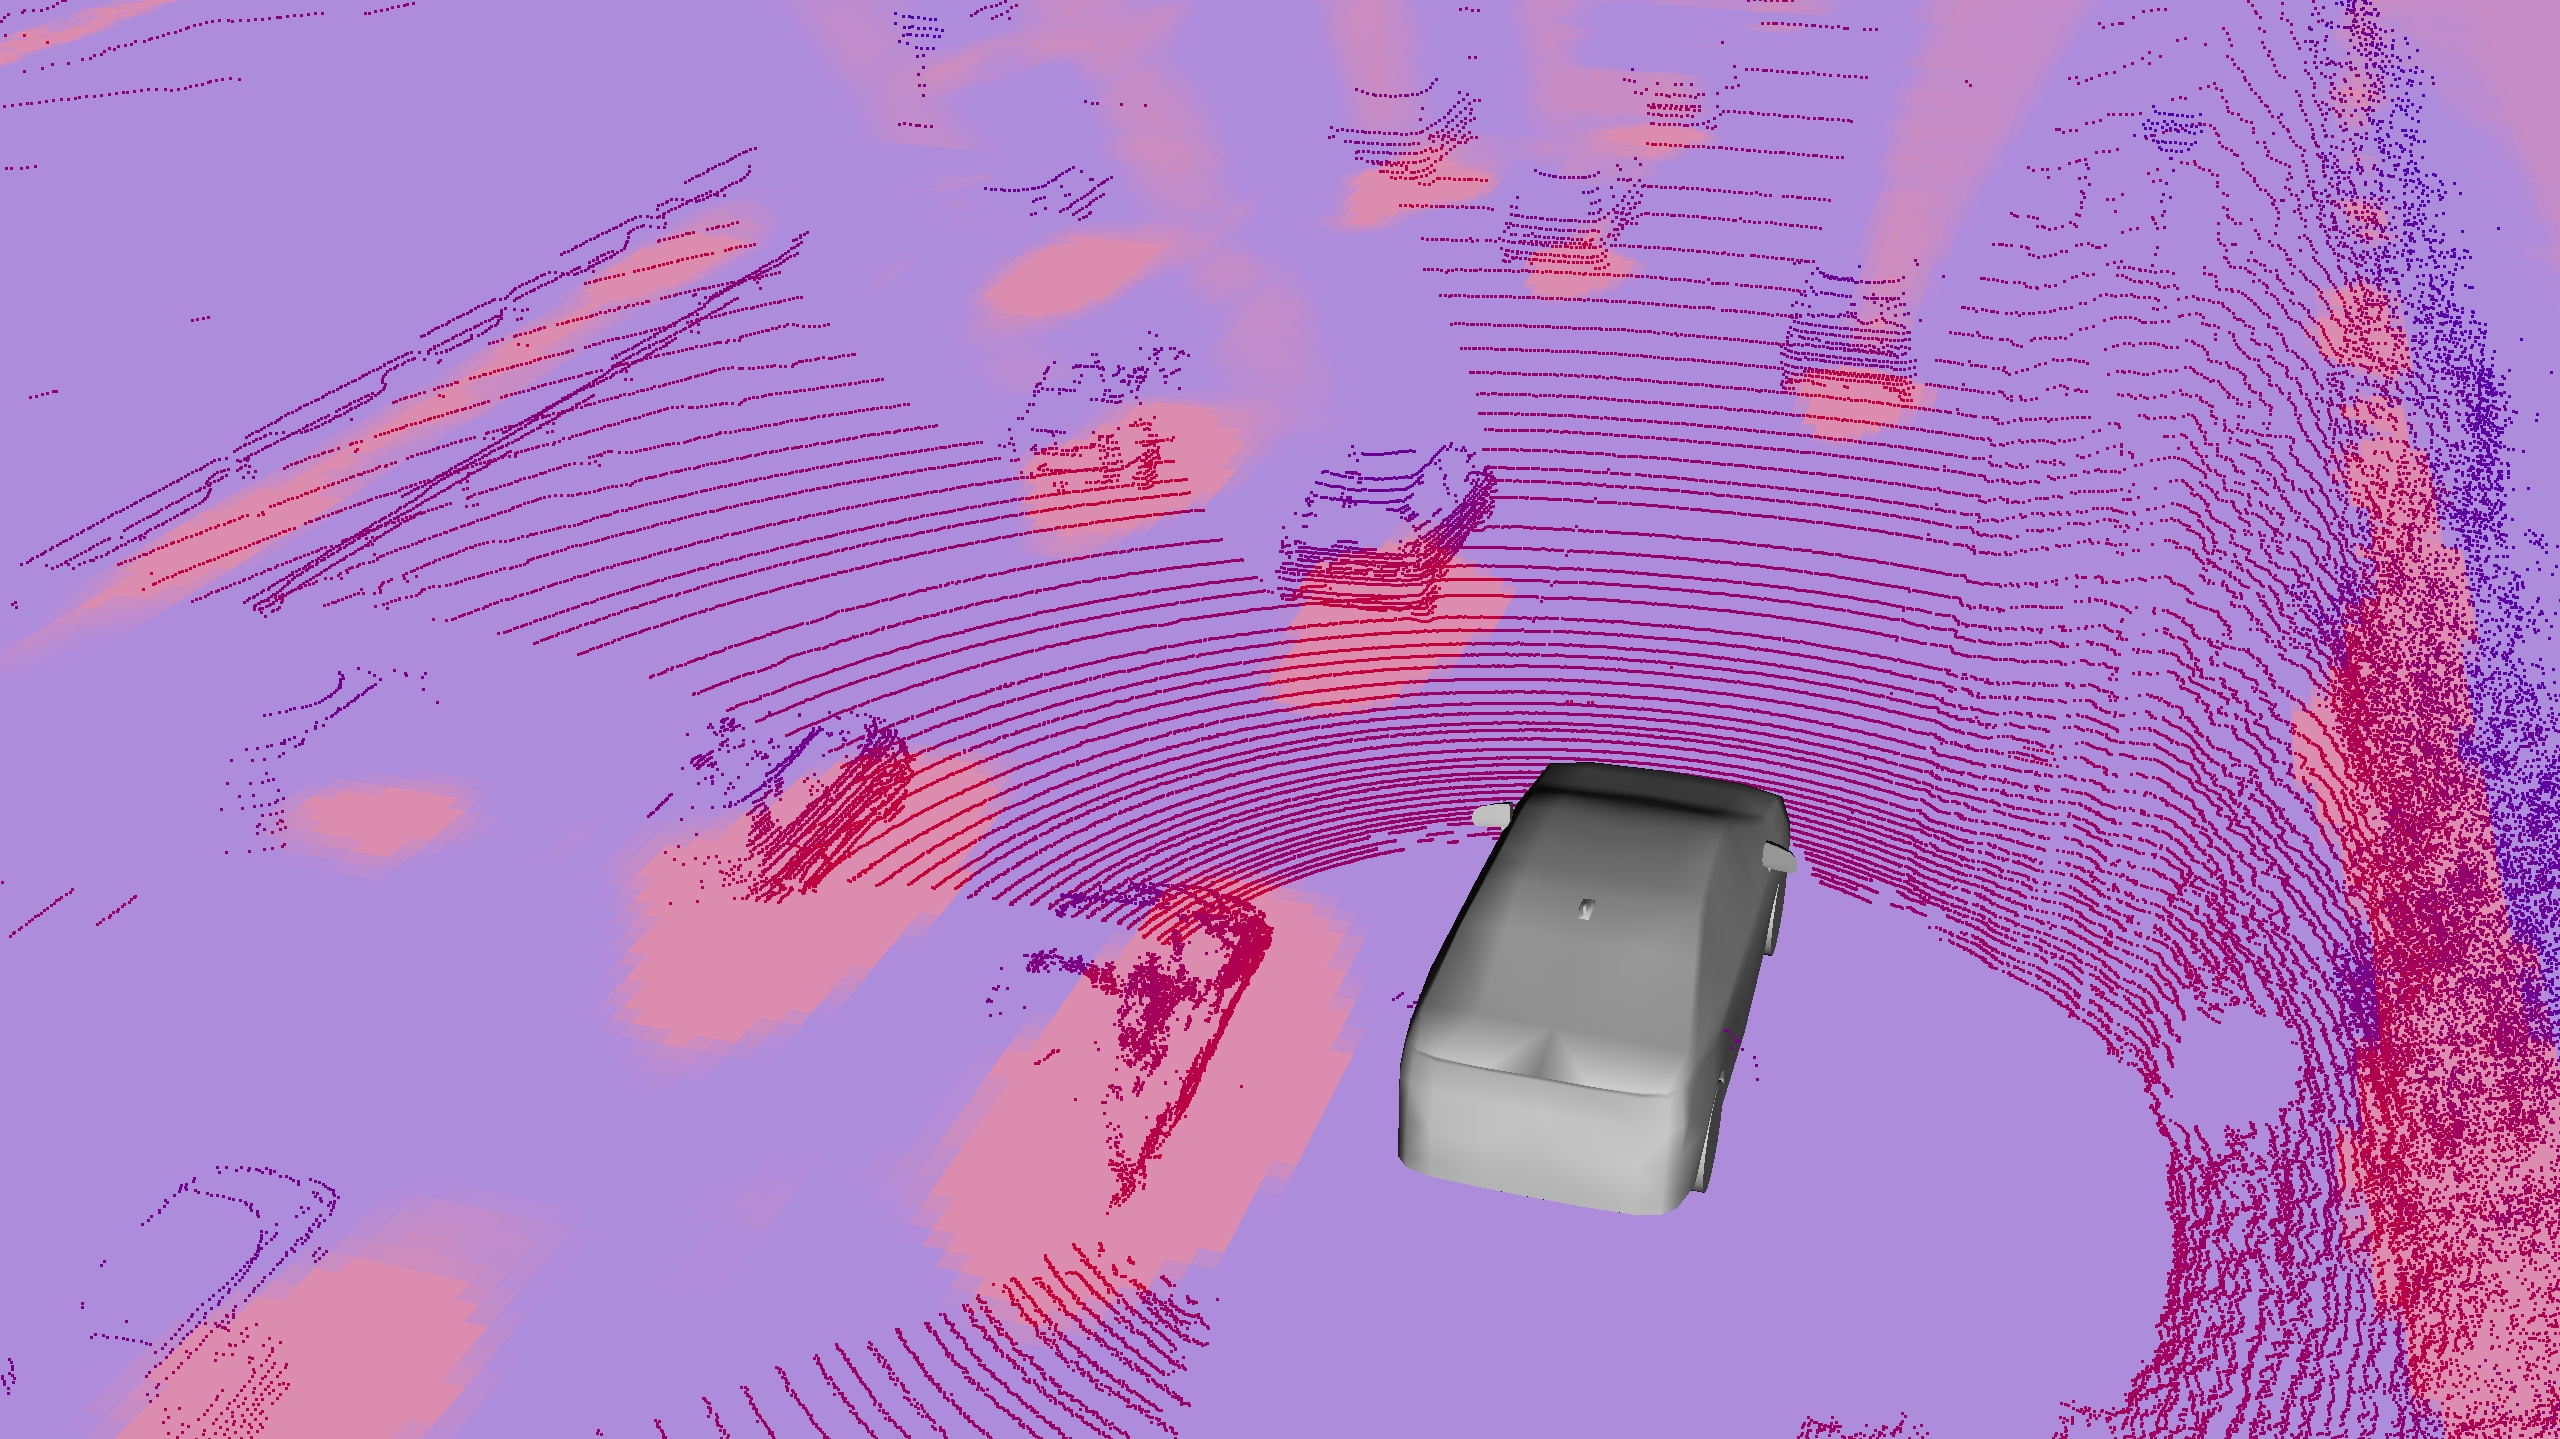
\includegraphics[width=\columnwidth]{figures/ex3.jpg}
  \caption{An example with both good detections and false positives on the
    background structure on either side of the road. Car likelihoods are shown
    in red.}
  \label{fig:ex3}
\end{figure}

%\section{Discussion and Future Work} \label{sec:discussion}

While the generated detection maps show some promising results, they do exhibit
many false positives. The models considered here are not able to differentiate
between certain background structure (such as vertical walls) and objects such
as cars.

In the future, it will be interesting to more closely compare these approaches
with that of \citep{wang2015RSS} or \citep{Engelcke2017ICRA}. Both of these
methods are similar to ours in that they used gridded \ac{LIDAR} observations
and shape features (although we additionally use free space). Perhaps
investigating these methods more closely will shed light on how to eliminate the
false positive detections on background structure. Perhaps this is due to their
training scheme, in which they perform hard negative mining to actively harvest
difficult background examples.

Furthermore, there are different ways of evaluating the observation model. While
we present a probabilistic method here, the literature provides many other
techniques. In object recognition, deep learning is commonly used to classify an
occupancy-grid-like representation of some object. While a large network might
prove intractable to rely on for evaluate \eqref{eq:detection_map} exhaustively,
investigating these methods more closely might provide value insight.
Alternatively, perhaps we could find some structure to exploit in the evaluation
of these models to improve runtime performance when they are repeatedly
evaluated, much like the sparse voting scheme in \citet{wang2015RSS} or the
implementation of separable kernels.

Longer term, it would be interesting to investigate how to apply this
representation temporally and evolve the detection map as sequences of
\ac{LIDAR} scans are taken. This could perhaps be integrated with an approach
such as \cite{ushani2017ICRA} and could possibly allow for tracking under
occlusion.

%\section{Conclusion}\label{sec:conclusion}

We have presented an approach that is a blend between occupancy mapping and
object detection, allowing for the generation of probabilistic object detection
maps. These maps not only capture object detections, but also capture regions
where objects are known to be absent, or areas where there is uncertainty. The
Bayesian framework that is used here is easily amendable to incorporating other
sensor measurements, such as from a multi-modal platform that includes camera,
and temporal propagation of the detection map to capture the dynamics of the
scene. We have investigated a few different ways to evaluate the observation
models for this method, though each is subject to false positives. However, we
believe the high-level motivation of the work is valuable, and in the future we
will consider further developing these models to alleviate the presented issues.

The code for this work is available at https://bitbucket.org/aushani/summer.


%\footnotesize
%\balance
%\bibliographystyle{IEEEtranN}
%\bibliography{strings-short,ieee-abrv,IEEE,references,library}

% that's all folks
\end{document}
